%%%%%%%%%%%%%%%%%%%%%%%%%%%%%%%%%%%%%%%%%%%%%%%%%%%%%%%%%%%%%%%%%%%%%%%%%%%%%%%
\section{The MoEDAL experiment at CERN}
\label{sec:exp}
%%%%%%%%%%%%%%%%%%%%%%%%%%%%%%%%%%%%%%%%%%%%%%%%%%%%%%%%%%%%%%%%%%%%%%%%%%%%%%%
%%=============================================================================
%\subsection{The LHC's magnificent seventh}
%\label{sec:moedalexpintro}
%%=============================================================================
In December 2009, the CERN Research Board approved the
\acs{LHC}'s seventh experiment -- the
Monopole and Exotics Detector at the LHC,
also known as \acs{MoEDAL}~\cite{MoEDAL2009}.
%
Housed in the same underground cavern as
the \acs{LHCb}~\cite{LHCb2008} experiment at
Interaction Point 8 (see Figure~\ref{fig:moedallhcbsim}),
\ac{MoEDAL} continues the collider-based search for magnetic monopoles
at today's particle physics energy frontier:
the proton-proton collisions of the \ac{LHC}.
Like all \ac{LHC} experiments,
the scientific work -- installing and running the detectors,
processing the data, and publishing the results -- is done by the
\ac{MoEDAL} Collaboration.
\acs{IRIS} is a member of the \ac{MoEDAL} Collaboration,
and so -- by being a member of \ac{IRIS} -- you are too!

%
\begin{figure}[htbp]
  \centering
  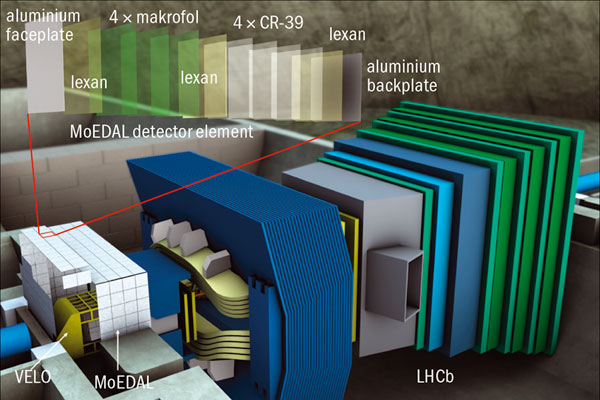
\includegraphics[width=1.0\textwidth]{assets/images/moedallhcbsim/moedallhcbsim.jpg}
  \caption[The MoEDAL experiment in the LHCb cavern]
  {\label{fig:moedallhcbsim}The \ac{MoEDAL} experiment in the \ac{LHCb} %
cavern, with the \ac{LHCb} detector (and \ac{VeLo} subdetector) shown for %
context.  The structure of a \ac{MoEDAL} \acf{NTD} element is shown %
in the exploded inset image. Image credit: \href{http://moedal.web.cern.ch}{The MoEDAL Collaboration}; %
please contact them regarding licensing/re-use of this image.}
\end{figure}
%

The first test detector elements of the \ac{MoEDAL} experiments were
installed in 2009, just before the \ac{LHC} was restarted following its
2008 malfunction.
%
The first full stack of Nuclear Track Detectors (NTDs – see below) were
put in place in January 2011, and officially began taking data on the
3rd of June 2015.
%
Since the publication of the \ac{MoEDAL} \ac{TDR} in 2009~\cite{MoEDAL2009},
however, the \ac{MoEDAL} experiment has grown and evolved to incorporate
additional subdetector systems to improve the chances of discovering a
magnetic monopole (or sign of physics beyond the Standard Model).
Let's take a look at these now.

%%=============================================================================
%\subsection{The subdetector systems}
%\label{sec:moedalsubdet}
%%=============================================================================

%-----------------------------------------------------------------------------
\subsection{The Nuclear Track Detectors}
\label{sec:ntds}
%-----------------------------------------------------------------------------
The \ac{MoEDAL} design concept was initially based only on the use of
devices known as \acfp{NTD}, following in the footsteps of the last monopole
searches carried out in CERN's 27km underground tunnel~\cite{Pinfold2009}.
\acp{NTD} are essentially sheets of material that, when hit with a massive,
highly-ionizing particle (\acs{HIP}), get damaged in such a way that we can 
analyse the damage and infer properties of whatever caused it.
%
For example, in the CR-39 \textregistered{} plastic used by \ac{MoEDAL},
\acp{HIP} break bonds in the plastic's hydrocarbons along the path of
the \ac{HIP}.
%
Careful etching with sodium hydroxide (NaOH) forms conical pits in the 
surface of the plastic along these paths, and by analysing the size, 
shape and angle of the cones we can learn more about the particle that 
caused them. \ac{MoEDAL} uses four types of \ac{NTD} material:
Lexan, Makrofol, and CR-39~\textregistered, each of which have different
sensitivities to the \ac{HIP}'s charge and momentum.
These can be seen in the exploded inset image in Figure~\ref{fig:moedallhcbsim}
(schematic) and the top-left of Figure~\ref{fig:ntd} (actual sheets).
Recently, additional sheets of Makrofol have been added within the \ac{LHCb}
experiment itself in the form of the \ac{VHCC} in order to increase the 
chances of spotting a monopole.

%
\begin{figure}[htbp]
  \centering
  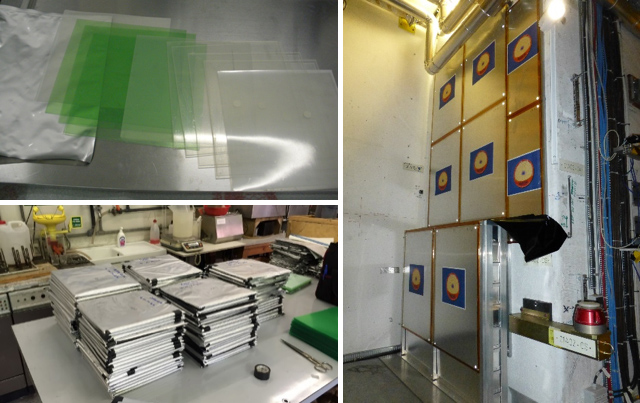
\includegraphics[width=1.0\textwidth]{assets/images/ntd/ntd.jpg}
  \caption[The MoEDAL Nuclear Track Detectors]
  {\label{fig:ntd}The component sheets of a MoEDAL \acf{NTD} stack (top-left); %
\ac{MoEDAL} \ac{NTD} stacks ready for deployment in the \ac{LHCb} cavern (bottom-left), %
and; some of the \ac{MoEDAL} \acp{NTD} in situ (right).  %
Image credit: \href{http://moedal.web.cern.ch}{R. Soluk/The MoEDAL Collaboration}; please contact them regarding licensing/re-use of this image.}
\end{figure}
%

In many ways, \acp{NTD} are like the nuclear emulsions used by particle
physicists in the 1950s in cosmic ray and early accelerator experiments.
The use of such emulsions was pioneered by Cecil Powell,
who won the 1950 Nobel Prize for Physics for this technique and the
discoveries he made with it.
%
The passage of a charged particle through the emulsion would ionise the
sensitive particles in such a way that the application of a chemical
would produce a light-blocking substance along the path,
making it visible.
The same principle is used in film-based photography.
The key thing is the sensitivity of the particles in the emulsion;
Powell's silver iodide-based emulsions were great for discovering mesons
in balloon flights or up mountains,
but would be overwhelmed by the energy and intensity of what the
LHC's collisions produce.

Luckily, magnetic monopoles are predicted to be so highly-charged
that we can use something less sensitive, more stable, and a bit cheaper
to record the tracks they would leave behind.
While breaking hydrocarbon bonds in a plastic is a different physical process,
the principles are the same -- including those used in the analysis.
Terabytes of digital images of the etched plastic from \ac{MoEDAL} \ac{NTD}
stacks -- like those shown in Figure~\ref{fig:ntd} -- need to be checked
for the tell-tale tracks of the monopole.
Given the unknown nature of the signal we expect (and the complexity of the
proton-proton collision background),
we will need help to do this -- which is one of the ways you can help.

%-----------------------------------------------------------------------------
\subsection{The Magnetic Monopole Trapper}
\label{sec:mmt}
%-----------------------------------------------------------------------------
The \acf{MMT} goes one step further than the \acfp{NTD}.
Rather than just recording the passage of the monopole through the material --
like finding the footprints of an animal in the jungle -- the \acp{MMT}
literally aim to trap the monopole so that it can be taken away and
studied further.
The \ac{MMT} is made up of many bars of aluminium packed closely 
together in boxes that are put in the \ac{LHCb} cavern around the
Interaction Point (see Figure~\ref{fig:mmt}).
If we're lucky, magnetic monopoles passing through the aluminium would
slow down, stop, and become trapped within the aluminium. We can then 
carefully remove the bars from the cavern and pass them through a \acf{SQUID},
which would detect the monopole's magnetic charge~\cite{Mermod2014}.

%
\begin{figure}[htbp]
  \centering
  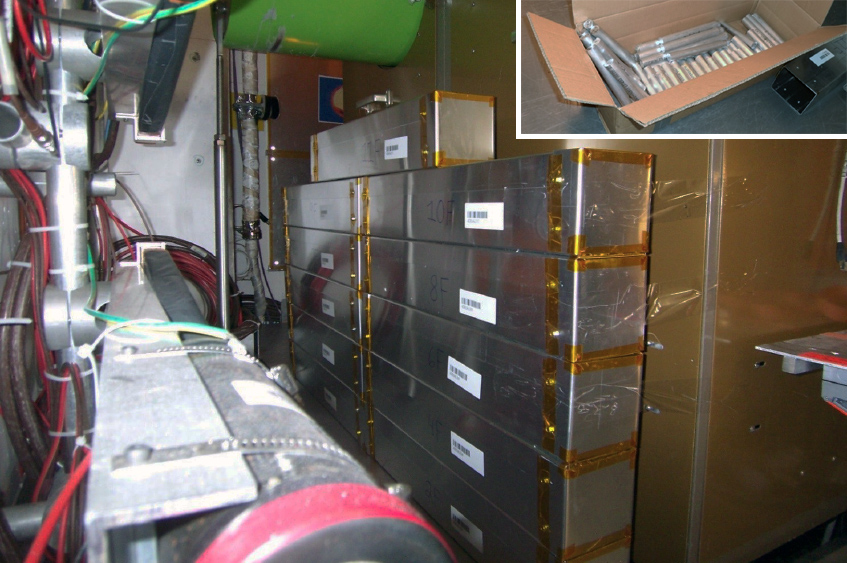
\includegraphics[width=1.0\textwidth]{assets/images/mmt/mmt.jpg}
  \caption[The MoEDAL Magnetic Monopole Trapper]
  {\label{fig:mmt}MoEDAL's prototype \acf{MMT} installed in the \ac{LHCb} cavern. %
Each box contains several bars of aluminium (see inset image, top-right) %
that are later removed from the cavern and scanned using a \ac{SQUID} %
to identify trapped magnetic monopoles.  %
Image credit: \href{http://moedal.web.cern.ch}{R. Soluk/The MoEDAL Collaboration}; %
please contact them regarding licensing/re-use of this image.}
\end{figure}
%

Finding a monopole this way would be particularly exciting,
as with the monopole embedded in the material of the detector we would 
have the chance to perform all sorts of studies to find out more about the 
properties of magnetic monopoles.  In fact, searches for trapped monopoles 
from collider experiments have been performed before using decommissioned detector 
and beam pipe elements.  The beauty of MoEDAL's \acp{MMT} is that they 
are purpose-built for monopole trapping, and we don't have to wait for \acs{CMS}
and \acs{ATLAS} to finish their work and throw their kit away!

%-----------------------------------------------------------------------------
\subsection{The MoEDAL Timepix array}
\label{sec:timepixarray}
%-----------------------------------------------------------------------------
The particle collisions that take place during \ac{LHC} running -- with both
protons and lead ions -- produce a great deal of ionising radiation.
For the general-purpose \ac{LHC} experiments,
much of this is uninteresting in the sense that we understand its properties 
and studying it further will (generally speaking) not lead to new discoveries.
Signatures from these particles is known as ``background'' to the signal 
and needs to be filtered out from the data.
The \ac{MoEDAL} \acp{NTD} and \acp{MMT} are only sensitive to highly-ionising 
particles (\acp{HIP}) like monopoles, and so in principle do not need to 
worry about this background.
%
That said, it is important to double-check this assertion by measuring 
the background radiation in the \acs{LHCb} cavern. To this end, a number 
of Timepix hybrid silicon pixel detectors~\cite{Timepix2007, Timepix2008Erratum}
have been installed in the vicinity of \acs{LHCb}'s \acf{VeLo}.
The location of each device is shown in Figure~\ref{fig:tpx}.
\acs{IRIS} has access to data from these detectors -- which are of course the same 
detectors as used in the CERN@school detector network, LUCID, and the 
\acf{ISS}. Discovering something like a magnetic monopole would be an 
extraordinary discovery, and so demonstrating that we understand any possible 
backgrounds would be an essential part of verifying the discovery.
% before we 
%all get on the plane to Stockholm.

%
\begin{figure}[htbp]
  \centering
  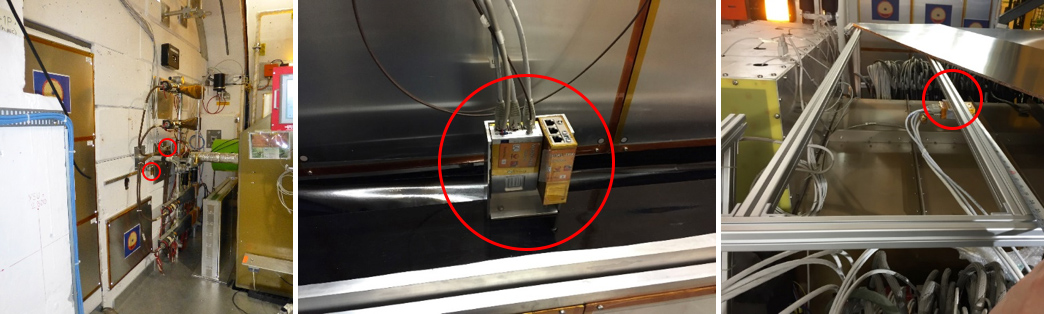
\includegraphics[width=1.0\textwidth]{assets/images/tpx/tpx.jpg}
  \caption[The MoEDAL Timepix detector array]
  {\label{fig:tpx}MoEDAL's five Timepix devices deployed around the %
\acs{LHCb} \acs{VeLo}. In the left-most image, TPX2 (TPX4) is shown %
in the lower-left (upper-right) red circle, where it has been installed %
with the sensor plane normal (parallel) to the beam pipe. %
In the central image, TPX1 (TPX3) is shown on the left (right) where it %
has been installed on the side of the \acs{VeLo} enclosure with the sensor %
plane normal (parallel) to the beam pipe. In the right-most image, TPX5 %
is shown installed above the \acs{VeLo} enclosure with the sensor plane %
normal to the beam pipe. %
Image credit: \href{http://moedal.web.cern.ch}{R. Soluk/The MoEDAL Collaboration}; %
please contact them regarding licensing/re-use of this image.}
\end{figure}
